
\chapter{Systematic Uncertainties}
\label{chap:Uncertainties}

\indent Systematic uncertainties can be separated into two categories, experimental uncertainties and theoretical uncertainties.  Experimental systematics result from uncertainties in physics object reconstruction, calibration, the understanding of the detectors and the amount of additional pile-up interactions.  Theoretical systematics result from uncertainties in PDFs, interaction scales, and theoretical calculations. Experimental uncertainties such as jet energy resolution are assumed to be 100 percent correlated across different background sources.  On the other hand, theoretical uncertainties are assumed to be uncorrelated from one another.  \\

\indent In general systematic uncertainties are parameterized as independent parameters with gaussian constraints.  These parameters are called ``nuisance'' parameters and normally denoted by the symbol $\alpha$.  The systematic errors on backgrounds are evaluated through a simultaneous fit to the control and signal regions.  An estimate of the systematic uncertainties on backgrounds in the signal region can be made by fitting to the control region alone and extrapolating the result to the signal region.  It is important to note that the fit can also lead to correlations between initially independent systematics uncertainties. \\

%\indent The amount of MC background in both the control and signal regions will vary with experimental and theoretical systematics before the fit.  However after the fit the total amount of background will be normalized to the control region.  If the MC yield for background has a downward variation for a given systematic then the normalization scale factor will increase.  The increased normalization scale factor will compensate for the simultaneous drop in the signal region MC yield.  This partial cancelation of fluctuations between control region and signal region can lead to smaller systematic uncertainties.  In effect, the control region reduces systematic uncertainty by directly measuring the amount of background in data instead of relying solely on MC simulations.\\

%If the background prediction varies in the same way in the control region and the signal region the total systematic in the signal region is partially canceled out in the transfer factor.  

\indent A control region that is kinematically similar to the signal region leads to cancelations of systematic uncertainties.  Because of this, designing a control region that is kinematically similar to the signal region is crucial to mitigating systematic uncertainties.  More detail on control region design and systematic uncertainties can be found in chapter \ref{sec:Bkg:Tech} on background estimation and chapter \ref{chap:statistics} on statistical analysis.  \\

%\indent The fit may compensate for a change in one systematic by varying several other systematics in order to get the best fit in the control region.  The correlation matrix between a reduced set of systematic variations and background scale factor after the simultaneous fit to all control regions are given in figure \ref{figure.corrMatrix}.

%\indent The fit can also lead to correlations between systematics that are initially parameterized as independent nuisance parameters before the fit to the control region.    The scale factor $\mu$ is the amount that the expected background MC must be scaled up/down by so that data and MC yields agree in the control region.  \\

\indent The total background systematic uncertainty is $\sim20\%$ in the signal region.  The dominant background systematic uncertainties in the first four signal region $\RISR$ bins, between $0.3 < \RISR < 0.7$, include uncertainty on the $\ttbar$ ISR/FSR, uncertainty on the $\ttbar$ matrix element and parton shower calculation, and uncertainty on the jet energy resolution.  Each of these dominant systematic uncertainties contributes 5-10\% to the total uncertainty on background rate in the signal region.  The theoretical uncertainty on the amount of interference between SM $\ttbar$ and single top at NLO is also significant.  \\

\indent The large systematic uncertainty in the highest $\RISR$ bin between $0.7-0.8$ is completely due to low MC statistics caused by the low expected yield.  However the $0.7-0.8$ $\RISR$ region is completely statistically dominated for the same reason, with only 0.7 expected background events.  \\

\indent The dominant background uncertainties in each signal region bin is given in Table \ref{table.results.bkgestimate.uncertainties.SRC1_SRC2_SRC3}. \\% and \ref{table.results.bkgestimate.uncertainties.SRC4_SRC5}.  \\

%\begin{table}[htpb]
  %\caption{5 Largest Systematic Uncertainty on SM background in the Signal Region. }
  % \label{tab:sys:summary}
 % \begin{center}
 %   \def\arraystretch{1.4}%
 %   \begin{tabular}{c|c|c|c|c|c} \hline\hline
%      {\bf $\RISR$ region} &  0.3-0.4 & 0.4-0.5 & 0.5-0.6 & 0.6-0.7 & 0.7-0.8  \\ \hline 
%    \end{tabular}
 % \end{center}
%\end{table}%


\begin{table}
\caption[Breakdown of statistical and systematic uncertainty on background estimates]{
Breakdown of the dominant systematic uncertainties on background estimates.
Note that the individual uncertainties can be correlated, and do not necessarily add up quadratically to 
the total background uncertainty. The percentages show the size of the uncertainty relative to the total expected background.
\label{table.results.bkgestimate.uncertainties.SRC1_SRC2_SRC3}}
\begin{center}
\setlength{\tabcolsep}{0.0pc}
\begin{tabular*}{\textwidth}{@{\extracolsep{\fill}}lccc}
\noalign{\smallskip}\hline\noalign{\smallskip}
{\bf Uncertainty of channel}                                    & SRC1            & SRC2            & SRC3            \\
\noalign{\smallskip}\hline\noalign{\smallskip}
%%
Total background expectation             &  $20.56$        &  $27.54$        &  $18.86$       \\
%% \\
\noalign{\smallskip}\hline\noalign{\smallskip}
%%
Total statistical $(\sqrt{N_{\rm exp}})$              & $\pm 4.53$        & $\pm 5.25$        & $\pm 4.34$       \\
%%
Total background systematic               & $\pm 6.62\ [32.18\%] $        & $\pm 4.89\ [17.75\%] $        & $\pm 3.53\ [18.72\%] $             \\
\noalign{\smallskip}\hline\noalign{\smallskip}
\noalign{\smallskip}\hline\noalign{\smallskip}
%%
ttbar ME/PS uncertainty         & $\pm 4.86\ [23.6\%] $          & $\pm 1.91\ [6.9\%] $          & $\pm 2.39\ [12.7\%] $       \\
%%
ISR/FSR uncertainty                                & $\pm 2.64\ [12.8\%] $          & $\pm 2.19\ [8.0\%] $          & $\pm 1.06\ [5.6\%] $       \\
%%
Single Top Theory Uncertainty          & $\pm 1.66\ [8.1\%] $          & $\pm 1.18\ [4.3\%] $          & $\pm 1.21\ [6.4\%] $       \\
%%
MC statistics in SR bin        & $\pm 1.29\ [6.3\%] $          & $\pm 1.42\ [5.1\%] $            & $\pm 0.96\ [5.1\%] $       \\
%%
ttbar CR normalization factor         & $\pm 0.91\ [4.4\%] $          & $\pm 1.55\ [5.6\%] $          & $\pm 1.03\ [5.4\%] $       \\
%%
Jet energy resolution         & $\pm 0.81\ [3.9\%] $          & $\pm 2.70\ [9.8\%] $          & $\pm 1.14\ [6.0\%] $       \\
%%
QCD Jet Smearing Uncertainty        & $\pm 2.38\ [11.6\%] $          & $\pm 0.77\ [2.8\%] $          & $\pm 0.17\ [0.91\%] $       \\
%%
%alpha\_JET\_GroupedNP\_3         & $\pm 0.72\ [3.5\%] $          & $\pm 0.03\ [0.10\%] $          & $\pm 0.17\ [0.89\%] $       \\
%%
%mu\_SingleTop         & $\pm 0.56\ [2.7\%] $          & $\pm 0.40\ [1.4\%] $          & $\pm 0.41\ [2.2\%] $       \\
%%
%alpha\_MET\_SoftTrk\_ResoPerp         & $\pm 0.46\ [2.3\%] $          & $\pm 0.56\ [2.0\%] $          & $\pm 0.22\ [1.2\%] $       \\
%%
%alpha\_cEff         & $\pm 0.43\ [2.1\%] $          & $\pm 0.40\ [1.5\%] $          & $\pm 0.11\ [0.60\%] $       \\
%%
%alpha\_JET\_GroupedNP\_2         & $\pm 0.30\ [1.5\%] $          & $\pm 0.78\ [2.8\%] $          & $\pm 0.36\ [1.9\%] $       \\
%%
%alpha\_JET\_GroupedNP\_1         & $\pm 0.27\ [1.3\%] $          & $\pm 0.06\ [0.23\%] $          & $\pm 0.04\ [0.19\%] $       \\
%%
%alpha\_MET\_SoftTrk\_Scale         & $\pm 0.23\ [1.1\%] $          & $\pm 0.29\ [1.0\%] $          & $\pm 0.08\ [0.45\%] $       \\
%%
%alpha\_theoSysDiboson         & $\pm 0.19\ [0.94\%] $          & $\pm 0.10\ [0.37\%] $          & $\pm 0.14\ [0.76\%] $       \\
%%
%alpha\_CExtrap         & $\pm 0.16\ [0.80\%] $          & $\pm 0.31\ [1.1\%] $          & $\pm 0.19\ [1.0\%] $       \\
%%
%alpha\_LightEff         & $\pm 0.15\ [0.74\%] $          & $\pm 0.22\ [0.80\%] $          & $\pm 0.04\ [0.23\%] $       \\
%%
%alpha\_bEff         & $\pm 0.14\ [0.70\%] $          & $\pm 0.00\ [0.01\%] $          & $\pm 0.07\ [0.36\%] $       \\
%%
%alpha\_JET\_EtaNonClosure         & $\pm 0.11\ [0.54\%] $          & $\pm 1.13\ [4.1\%] $          & $\pm 0.01\ [0.03\%] $       \\
%%
%mu\_Wjets         & $\pm 0.09\ [0.45\%] $          & $\pm 0.22\ [0.81\%] $          & $\pm 0.22\ [1.2\%] $       \\
%%
%alpha\_theoSysW         & $\pm 0.09\ [0.45\%] $          & $\pm 0.24\ [0.88\%] $          & $\pm 0.23\ [1.2\%] $       \\
%%
%alpha\_MET\_SoftTrk\_ResoPara         & $\pm 0.07\ [0.35\%] $          & $\pm 0.19\ [0.68\%] $          & $\pm 0.03\ [0.15\%] $       \\
%%
%mu\_TtbarV         & $\pm 0.05\ [0.22\%] $          & $\pm 0.09\ [0.34\%] $          & $\pm 0.09\ [0.47\%] $       \\
%%
%alpha\_PILEUP         & $\pm 0.02\ [0.11\%] $          & $\pm 0.32\ [1.2\%] $          & $\pm 0.12\ [0.64\%] $       \\
%%
%alpha\_FTExtrap         & $\pm 0.02\ [0.11\%] $          & $\pm 0.04\ [0.13\%] $          & $\pm 0.03\ [0.17\%] $       \\
%%
%alpha\_theoSysTTbarV         & $\pm 0.01\ [0.07\%] $          & $\pm 0.03\ [0.11\%] $          & $\pm 0.03\ [0.15\%] $       \\
%%
%alpha\_JVT         & $\pm 0.01\ [0.06\%] $          & $\pm 0.04\ [0.13\%] $          & $\pm 0.04\ [0.22\%] $       \\
%%
%gamma\_stat\_SRC2\_cuts\_bin\_0         & $\pm 0.00\ [0.00\%] $          & $\pm 1.42\ [5.1\%] $          & $\pm 0.00\ [0.00\%] $       \\
%%
%gamma\_stat\_SRC3\_cuts\_bin\_0         & $\pm 0.00\ [0.00\%] $          & $\pm 0.00\ [0.00\%] $          & $\pm 0.96\ [5.1\%] $       \\
%%
\noalign{\smallskip}\hline\noalign{\smallskip}
\end{tabular*}

\begin{tabular*}{\textwidth}{@{\extracolsep{\fill}}lcc}
\noalign{\smallskip}\hline\noalign{\smallskip}
{\bf Uncertainty of channel}                                    & SRC4            & SRC5            \\
\noalign{\smallskip}\hline\noalign{\smallskip}
%%
Total background expectation             &  $7.69$        &  $0.90$       \\
%% \\
\noalign{\smallskip}\hline\noalign{\smallskip}
%%
Total statistical $(\sqrt{N_{\rm exp}})$              & $\pm 2.77$        & $\pm 0.95$       \\
%%
Total background systematic               & $\pm 1.37\ [17.77\%] $        & $\pm 0.71\ [78.68\%] $             \\
\noalign{\smallskip}\hline\noalign{\smallskip}
\noalign{\smallskip}\hline\noalign{\smallskip}
%%
ttbar ME/PS uncertainty        & $\pm 0.68\ [8.8\%] $          & $\pm 0.63\ [69.1\%] $       \\
%%
ISR/FSR uncertainty        & $\pm 0.46\ [6.0\%] $          & $\pm 0.13\ [14.8\%] $       \\
%%
Single Top Theory Uncertainty        & $\pm 0.71\ [9.3\%] $          & $\pm 0.00\ [0.00\%] $       \\
%%
MC statistics in SR bin         & $\pm 0.54\ [7.0\%] $          & $\pm 0.21\ [23.0\%] $         \\
%%
ttbar CR normalization factor         & $\pm 0.35\ [4.5\%] $          & $\pm 0.04\ [4.9\%] $       \\
%%
Jet Energy Resolution        & $\pm 0.35\ [4.6\%] $          & $\pm 0.09\ [9.7\%] $       \\
%%
QCD Jet Smearing Uncertainty        & $\pm 0.02\ [0.26\%] $          & $\pm 0.00\ [0.15\%] $       \\
%%
%mu\_SingleTop         & $\pm 0.24\ [3.1\%] $          & $\pm 0.00\ [0.00\%] $       \\
%%
%mu\_Wjets         & $\pm 0.22\ [2.9\%] $          & $\pm 0.02\ [2.7\%] $       \\
%%
%alpha\_theoSysW         & $\pm 0.21\ [2.7\%] $          & $\pm 0.02\ [2.3\%] $       \\
%%
%alpha\_JET\_GroupedNP\_1         & $\pm 0.18\ [2.3\%] $          & $\pm 0.04\ [4.2\%] $       \\
%%
%alpha\_PILEUP         & $\pm 0.15\ [2.0\%] $          & $\pm 0.13\ [13.9\%] $       \\
%%
%alpha\_MET\_SoftTrk\_ResoPerp         & $\pm 0.14\ [1.9\%] $          & $\pm 0.01\ [1.6\%] $       \\
%%
%alpha\_MET\_SoftTrk\_ResoPara         & $\pm 0.13\ [1.7\%] $          & $\pm 0.00\ [0.12\%] $       \\
%%
%alpha\_LightEff         & $\pm 0.12\ [1.6\%] $          & $\pm 0.02\ [1.9\%] $       \\
%%
%alpha\_bEff         & $\pm 0.08\ [1.0\%] $          & $\pm 0.01\ [1.4\%] $       \\
%%
%alpha\_cEff         & $\pm 0.07\ [0.93\%] $          & $\pm 0.03\ [3.2\%] $       \\
%%
%alpha\_JET\_EtaNonClosure         & $\pm 0.07\ [0.87\%] $          & $\pm 0.11\ [12.4\%] $       \\
%%
%alpha\_JET\_GroupedNP\_3         & $\pm 0.06\ [0.72\%] $          & $\pm 0.02\ [2.5\%] $       \\
%%
%alpha\_JVT         & $\pm 0.02\ [0.29\%] $          & $\pm 0.00\ [0.35\%] $       \\
%%
%alpha\_CExtrap         & $\pm 0.02\ [0.23\%] $          & $\pm 0.00\ [0.22\%] $       \\
%%
%mu\_TtbarV         & $\pm 0.01\ [0.17\%] $          & $\pm 0.01\ [1.1\%] $       \\
%%
%alpha\_JET\_GroupedNP\_2         & $\pm 0.01\ [0.15\%] $          & $\pm 0.09\ [10.3\%] $       \\
%%
%alpha\_FTExtrap         & $\pm 0.01\ [0.10\%] $          & $\pm 0.00\ [0.17\%] $       \\
%%
%lpha\_MET\_SoftTrk\_Scale         & $\pm 0.01\ [0.07\%] $          & $\pm 0.00\ [0.11\%] $       \\
%%
%gamma\_stat\_SRC5\_cuts\_bin\_0         & $\pm 0.00\ [0.00\%] $          & $\pm 0.21\ [23.0\%] $       \\
%%
\noalign{\smallskip}\hline\noalign{\smallskip}
\end{tabular*}

\end{center}
\end{table}
%
%
\begin{table}
\begin{center}
\setlength{\tabcolsep}{0.0pc}
\begin{tabular*}{\textwidth}{@{\extracolsep{\fill}}lcc}
\noalign{\smallskip}\hline\noalign{\smallskip}
{\bf Uncertainty of channel}                                    & SRC4            & SRC5            \\
\noalign{\smallskip}\hline\noalign{\smallskip}
%%
Total background expectation             &  $7.69$        &  $0.90$       \\
%% \\
\noalign{\smallskip}\hline\noalign{\smallskip}
%%
Total statistical $(\sqrt{N_{\rm exp}})$              & $\pm 2.77$        & $\pm 0.95$       \\
%%
Total background systematic               & $\pm 1.37\ [17.77\%] $        & $\pm 0.71\ [78.68\%] $             \\
\noalign{\smallskip}\hline\noalign{\smallskip}
\noalign{\smallskip}\hline\noalign{\smallskip}
%%
ttbar ME/PS uncertainty        & $\pm 0.68\ [8.8\%] $          & $\pm 0.63\ [69.1\%] $       \\
%%
ISR/FSR uncertainty        & $\pm 0.46\ [6.0\%] $          & $\pm 0.13\ [14.8\%] $       \\
%%
Single Top Theory Uncertainty        & $\pm 0.71\ [9.3\%] $          & $\pm 0.00\ [0.00\%] $       \\
%%
MC statistics in SR bin         & $\pm 0.54\ [7.0\%] $          & $\pm 0.21\ [23.0\%] $         \\
%%
ttbar CR normalization factor         & $\pm 0.35\ [4.5\%] $          & $\pm 0.04\ [4.9\%] $       \\
%%
Jet Energy Resolution        & $\pm 0.35\ [4.6\%] $          & $\pm 0.09\ [9.7\%] $       \\
%%
QCD Jet Smearing Uncertainty        & $\pm 0.02\ [0.26\%] $          & $\pm 0.00\ [0.15\%] $       \\
%%
%mu\_SingleTop         & $\pm 0.24\ [3.1\%] $          & $\pm 0.00\ [0.00\%] $       \\
%%
%mu\_Wjets         & $\pm 0.22\ [2.9\%] $          & $\pm 0.02\ [2.7\%] $       \\
%%
%alpha\_theoSysW         & $\pm 0.21\ [2.7\%] $          & $\pm 0.02\ [2.3\%] $       \\
%%
%alpha\_JET\_GroupedNP\_1         & $\pm 0.18\ [2.3\%] $          & $\pm 0.04\ [4.2\%] $       \\
%%
%alpha\_PILEUP         & $\pm 0.15\ [2.0\%] $          & $\pm 0.13\ [13.9\%] $       \\
%%
%alpha\_MET\_SoftTrk\_ResoPerp         & $\pm 0.14\ [1.9\%] $          & $\pm 0.01\ [1.6\%] $       \\
%%
%alpha\_MET\_SoftTrk\_ResoPara         & $\pm 0.13\ [1.7\%] $          & $\pm 0.00\ [0.12\%] $       \\
%%
%alpha\_LightEff         & $\pm 0.12\ [1.6\%] $          & $\pm 0.02\ [1.9\%] $       \\
%%
%alpha\_bEff         & $\pm 0.08\ [1.0\%] $          & $\pm 0.01\ [1.4\%] $       \\
%%
%alpha\_cEff         & $\pm 0.07\ [0.93\%] $          & $\pm 0.03\ [3.2\%] $       \\
%%
%alpha\_JET\_EtaNonClosure         & $\pm 0.07\ [0.87\%] $          & $\pm 0.11\ [12.4\%] $       \\
%%
%alpha\_JET\_GroupedNP\_3         & $\pm 0.06\ [0.72\%] $          & $\pm 0.02\ [2.5\%] $       \\
%%
%alpha\_JVT         & $\pm 0.02\ [0.29\%] $          & $\pm 0.00\ [0.35\%] $       \\
%%
%alpha\_CExtrap         & $\pm 0.02\ [0.23\%] $          & $\pm 0.00\ [0.22\%] $       \\
%%
%mu\_TtbarV         & $\pm 0.01\ [0.17\%] $          & $\pm 0.01\ [1.1\%] $       \\
%%
%alpha\_JET\_GroupedNP\_2         & $\pm 0.01\ [0.15\%] $          & $\pm 0.09\ [10.3\%] $       \\
%%
%alpha\_FTExtrap         & $\pm 0.01\ [0.10\%] $          & $\pm 0.00\ [0.17\%] $       \\
%%
%lpha\_MET\_SoftTrk\_Scale         & $\pm 0.01\ [0.07\%] $          & $\pm 0.00\ [0.11\%] $       \\
%%
%gamma\_stat\_SRC5\_cuts\_bin\_0         & $\pm 0.00\ [0.00\%] $          & $\pm 0.21\ [23.0\%] $       \\
%%
\noalign{\smallskip}\hline\noalign{\smallskip}
\end{tabular*}
\end{center}
\caption[Breakdown of uncertainty on background estimates]{
Breakdown of the dominant systematic uncertainties on background estimates.
Note that the individual uncertainties can be correlated, and do not necessarily add up quadratically to 
the total background uncertainty. The percentages show the size of the uncertainty relative to the total expected background.
\label{table.results.bkgestimate.uncertainties.SRC4_SRC5}}
\end{table}
%

%\begin{sidewaysfigure}[htbp]
%	\begin{center}
%		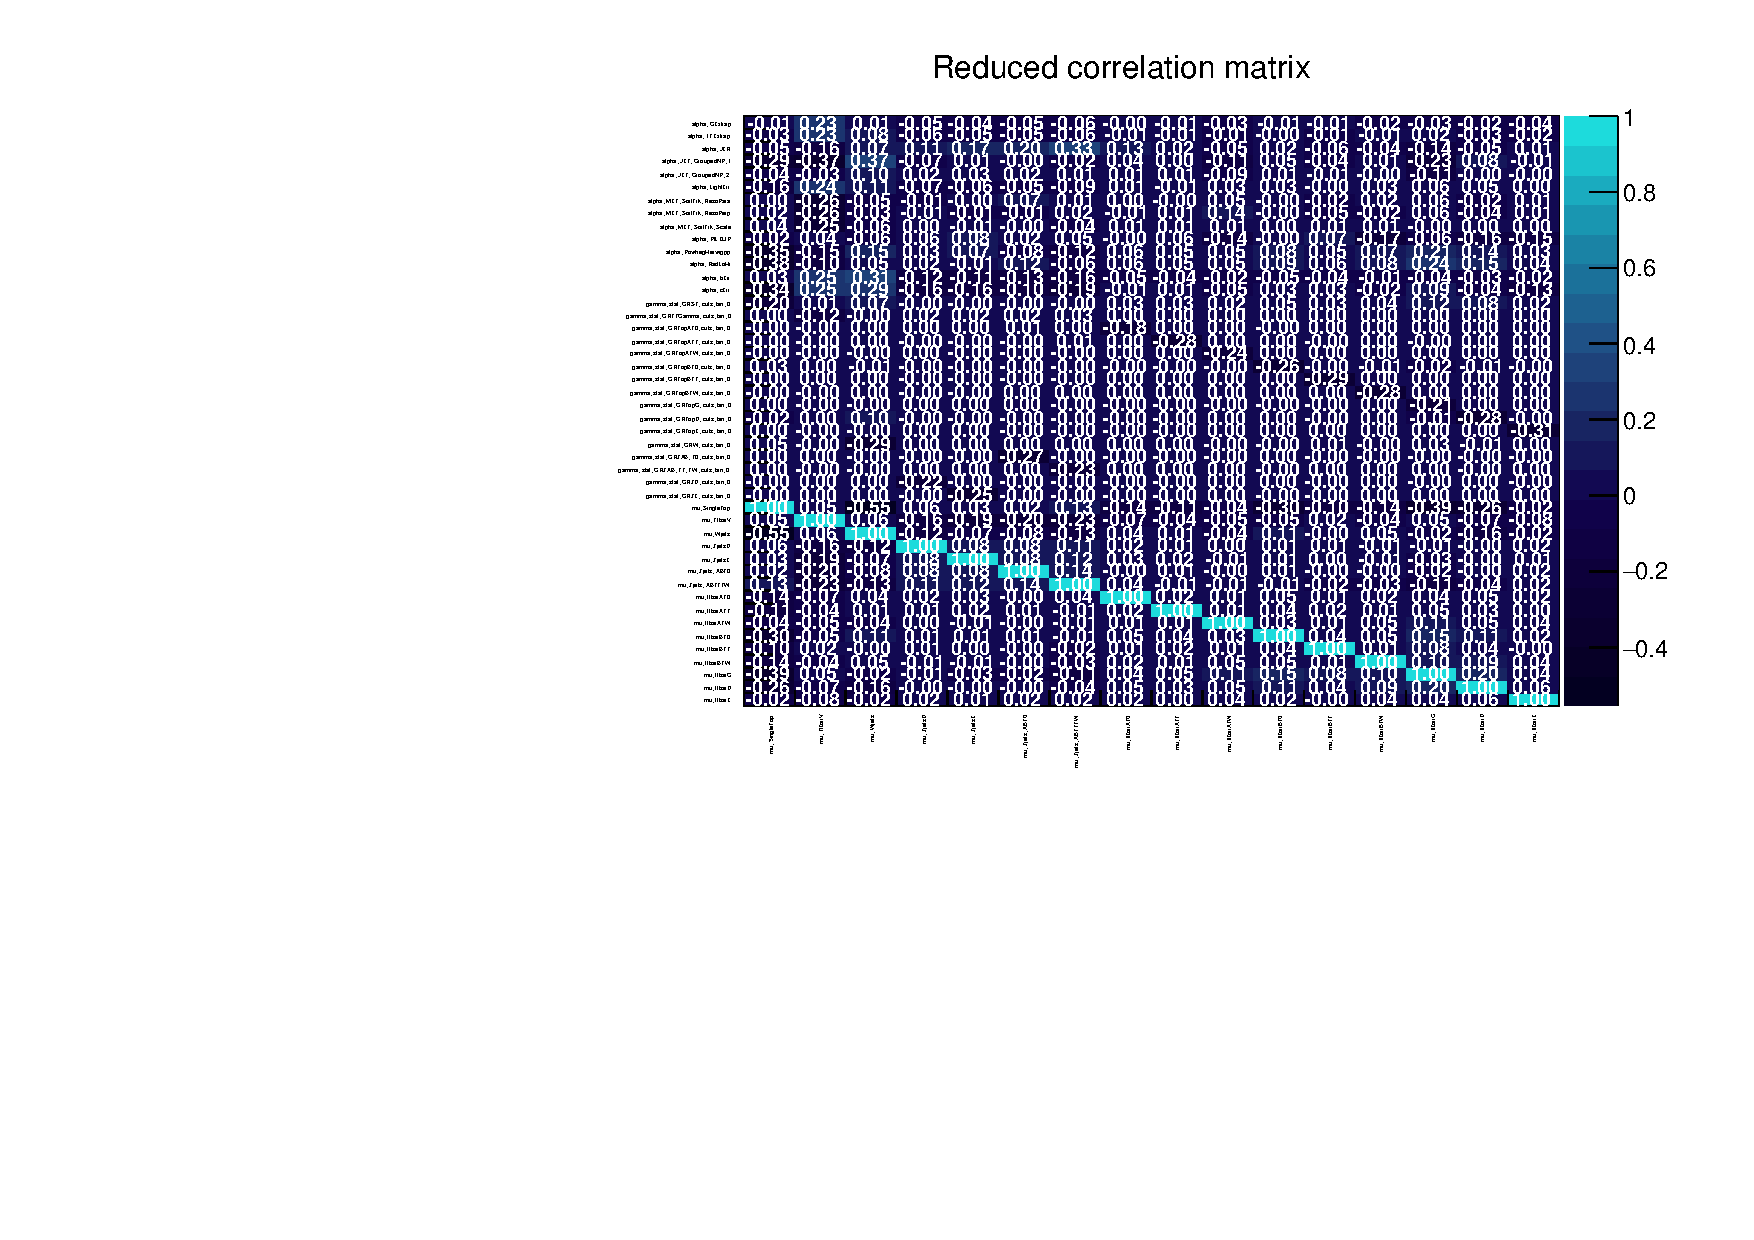
\includegraphics[width=0.85\textwidth, angle=90]{HistFitterStuff/corrMatrix.pdf}
%		\caption{Correlation matrix between select nuisance parameters.}
%		\label{figure.corrMatrix}
%	\end{center}
%\end{sidewaysfigure}

\indent The post background only fit pull is given in Figure \ref{figure.pullPlot}.  All nuisance parameters, $\alpha$, are close to zero with uncertainties close to plus/minus one.  No profiling of any systematics is observed. \\

\begin{figure}[h!]
	\begin{center}
		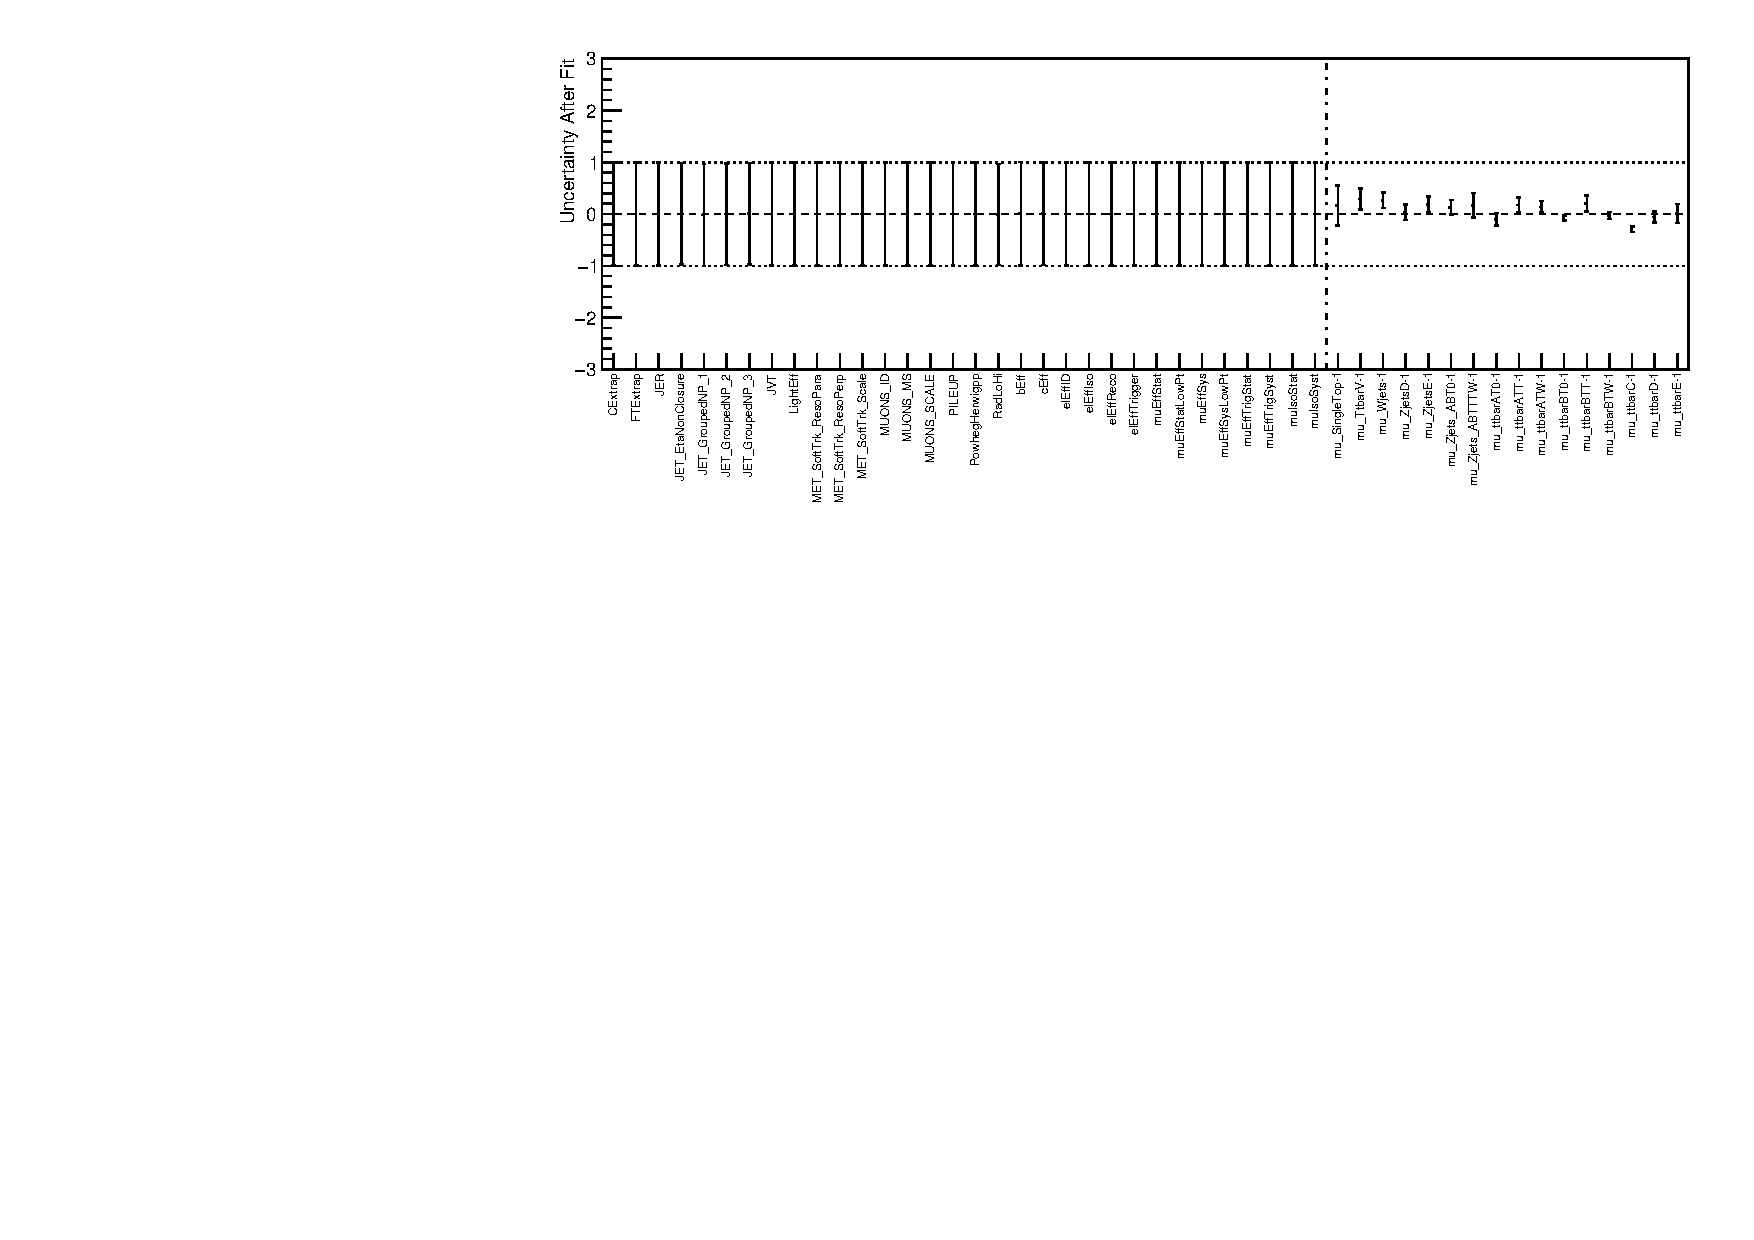
\includegraphics[width=0.45\textwidth, angle=180]{HistFitterStuff/pullPlot.pdf}
		\caption[Post-fit pull plot for the background-only fit]{Post-fit pull plot for the background-only fit.  All nuisance parameters ($\alpha$) are close to zero after the fit with a fit uncertainty close to plus/minus 1.  No profiling of any systematics is observed.  The background normalization factors to background control regions, $\mu$, are also shown.  Most background normalization factors are statistically consistent with the nominal value of 1.0 but mu\_ttbarC, the $\ttbar$ normalization in the $\ttbar$+hard ISR control region, has a central value of 0.707 and is inconsistent with 1.0.  This is because the $\ttbar$ MC overestimates the amount of $\ttbar$+hard ISR.   }
		\label{figure.pullPlot}
	\end{center}
\end{figure}

\indent A summary of the experimental and theoretical uncertainties relevant to this analysis is given in the sections below. \\

\subsection{Experimental Uncertainties}
\label{sec:ExpSystematics}

\indent Experimental systematics are estimated using a simultaneous fit of CR and the results extrapolated to the SR in a background only fit.  Variations on background yield and kinematics are determined by different object performance groups using a number of simulation based and data driven in-situ techniques.  A simultaneous fit to the CR gives the best fit value of the systematic parameter $\alpha$ and the systematic uncertainty associated with the background prediction in the SR. \\

\subsubsection*{Uncertainties on the Jet Energy Scale (JES) and Jet Energy Resolution (JER) } 

\indent The two main uncertainties affecting jet measurements are the uncertainties in JES and JER calibrations. The jet reconstruction and calibration process is described in section \ref{sec:reco:jets}.  Uncertainty in the calibration process leads to uncertainty in the calorimeter response to the true jet energy. \\

\indent Uncertainties on the JES are derived from different in-situ techniques by the ATLAS Jet/$\met$ group.  These techniques exploit the transverse momentum balance between a jet and a reference object such as a photon or a Z boson or between multiple jets in multijet events.\cite{JES_dijet, JES_ZGamma}.  The uncertainty on JES depends on $\eta$ and $\pt$ of the jet.  Uncertainties related to jet flavor composition and pile-up are also included.  \\

\indent  The ttbar control region require similar jet multiplicity and jet energy as the SR.  Therefore, much of the JES and JER uncertainties are canceled out in the transfer factor between the CR and SR.  Even after the cancelations, the JES uncertainty contributes around a 10 percent uncertainty to background yields and is one the major systematic uncertainties in this analysis.  \\

%\indent JES Uncertainty can be parameterized as a combination of 77 nuisance parameters.  This full set of nuisance parameter was combined to give a set of only 4 nuisance parameters.  The distribution of jets showed no dependence on the choice of full or reduced parameter set. \\

\indent The fractional JES uncertainty as a function of $\eta$ and $\pt$ for 2016 data can be see in figure \ref{fig:sys:JES}. \\

\begin{figure}[!htbp]
\begin{center}
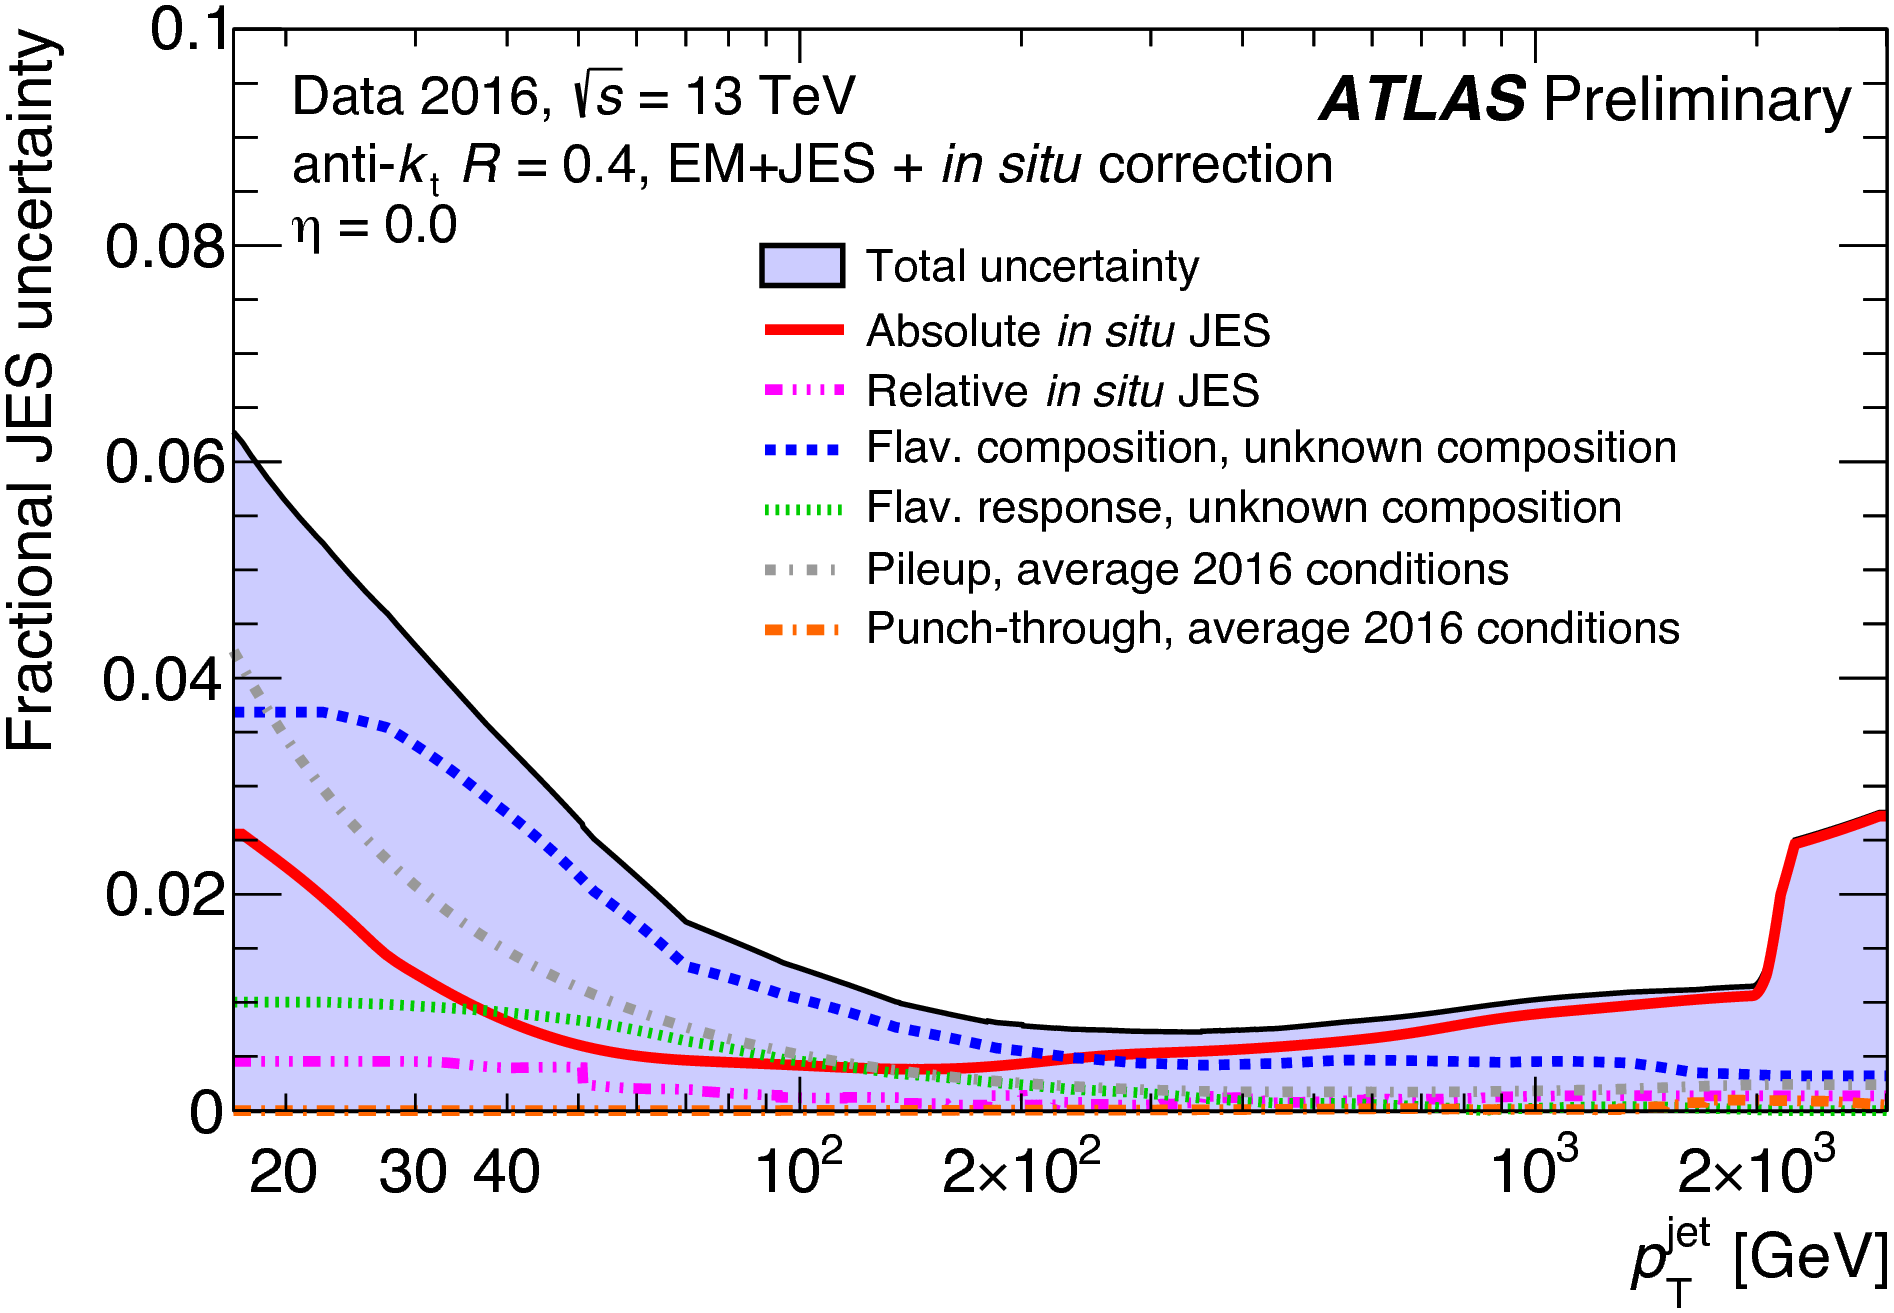
\includegraphics[width=0.48\textwidth]{figures/JetCalib/JES_pt.png}
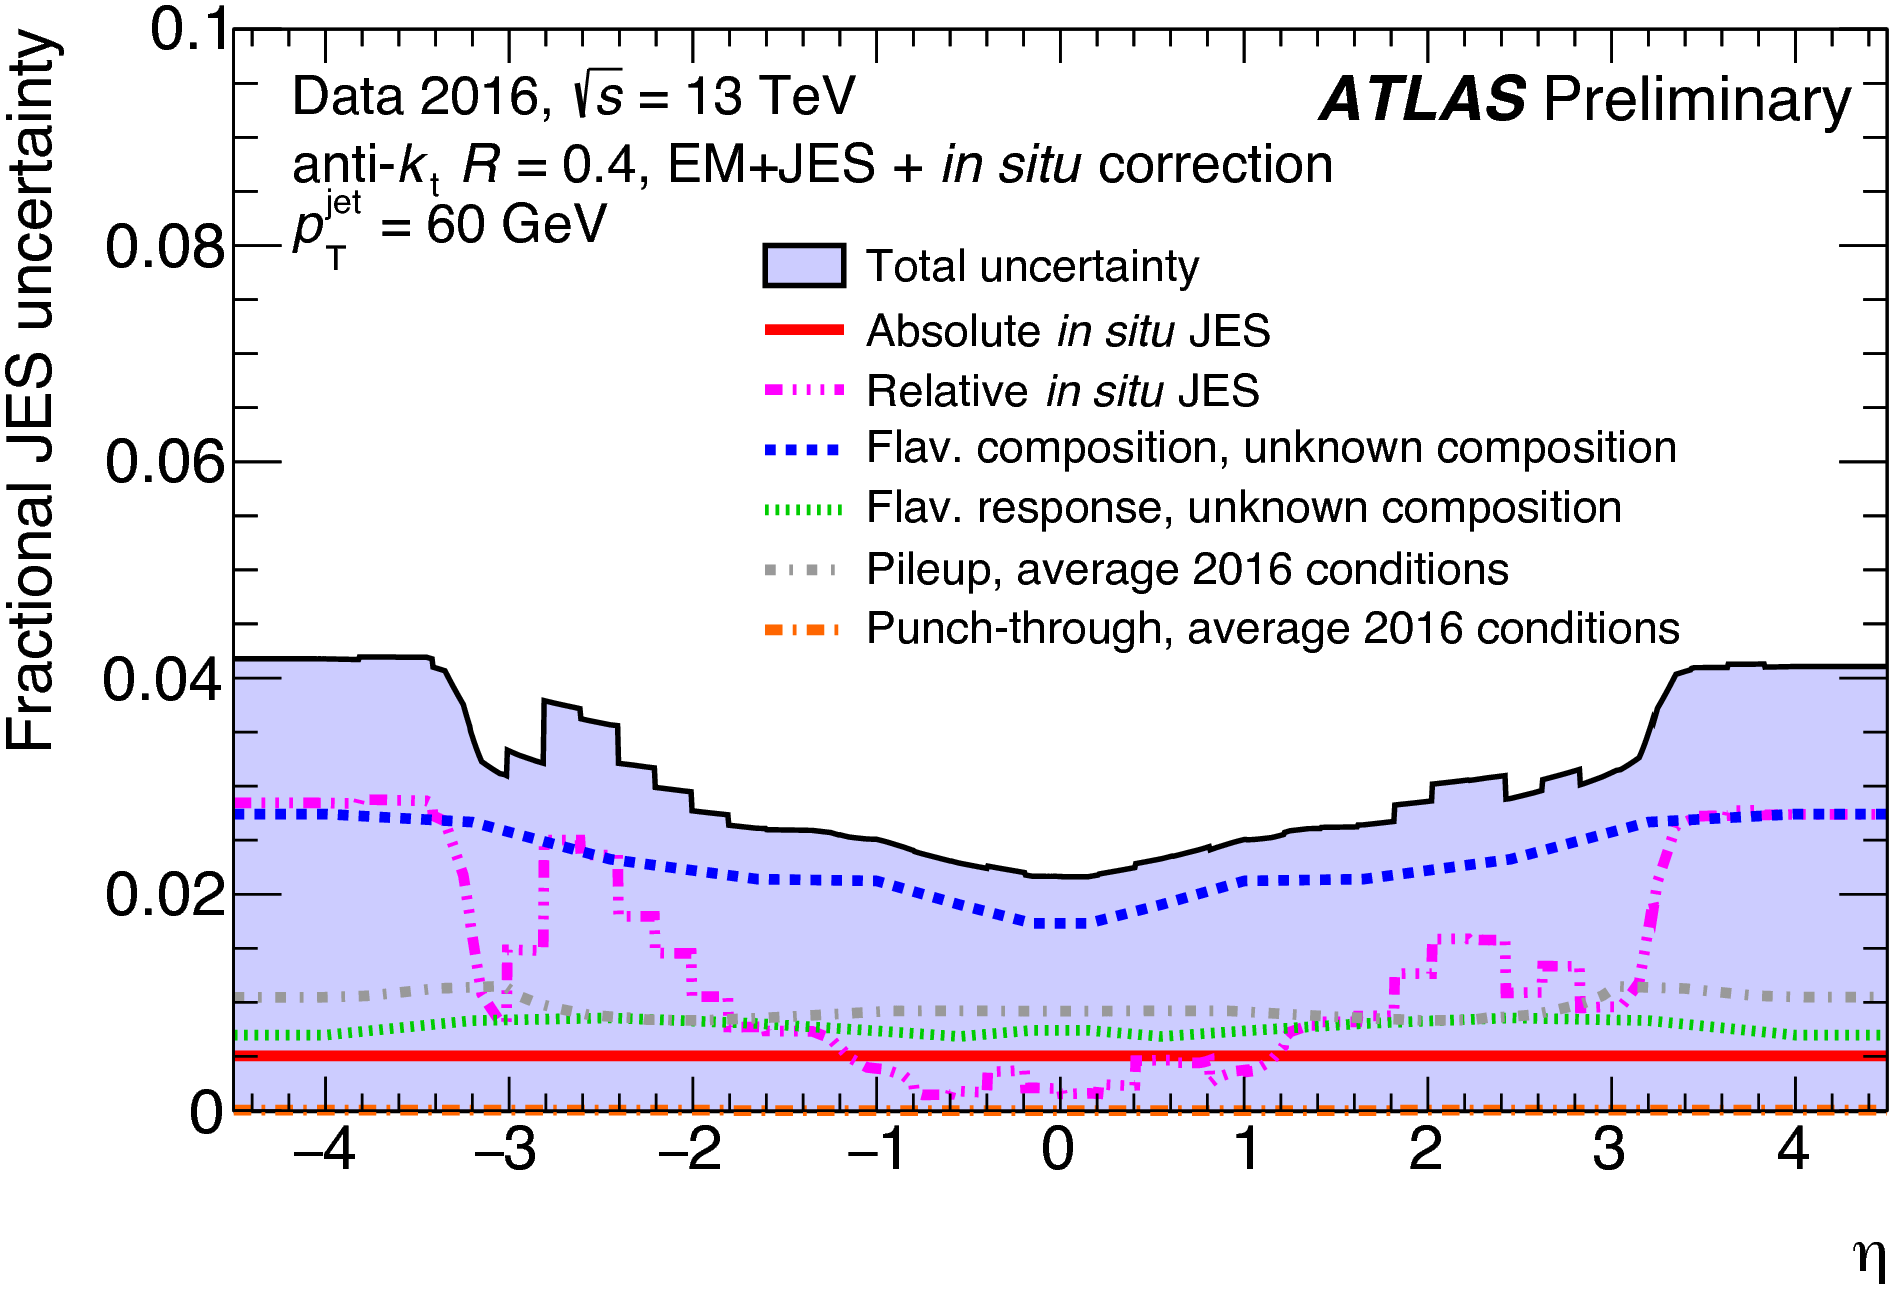
\includegraphics[width=0.48\textwidth]{figures/JetCalib/JES_eta.png}
\caption{Fractional uncertainty on the jet energy scale (JES) vs jet $\eta$ and jet $\pt$.  }
\label{fig:sys:JES}
\end{center}
\end{figure}

\indent Uncertainties on the JER are derived from dijet balance techniques.\cite{JES_dijet}  The fractional uncertainty on JER as a function of $\eta$ and $\pt$ can be seen in figure \ref{fig:sys:JER}\\

\begin{figure}[!htbp]
\begin{center}
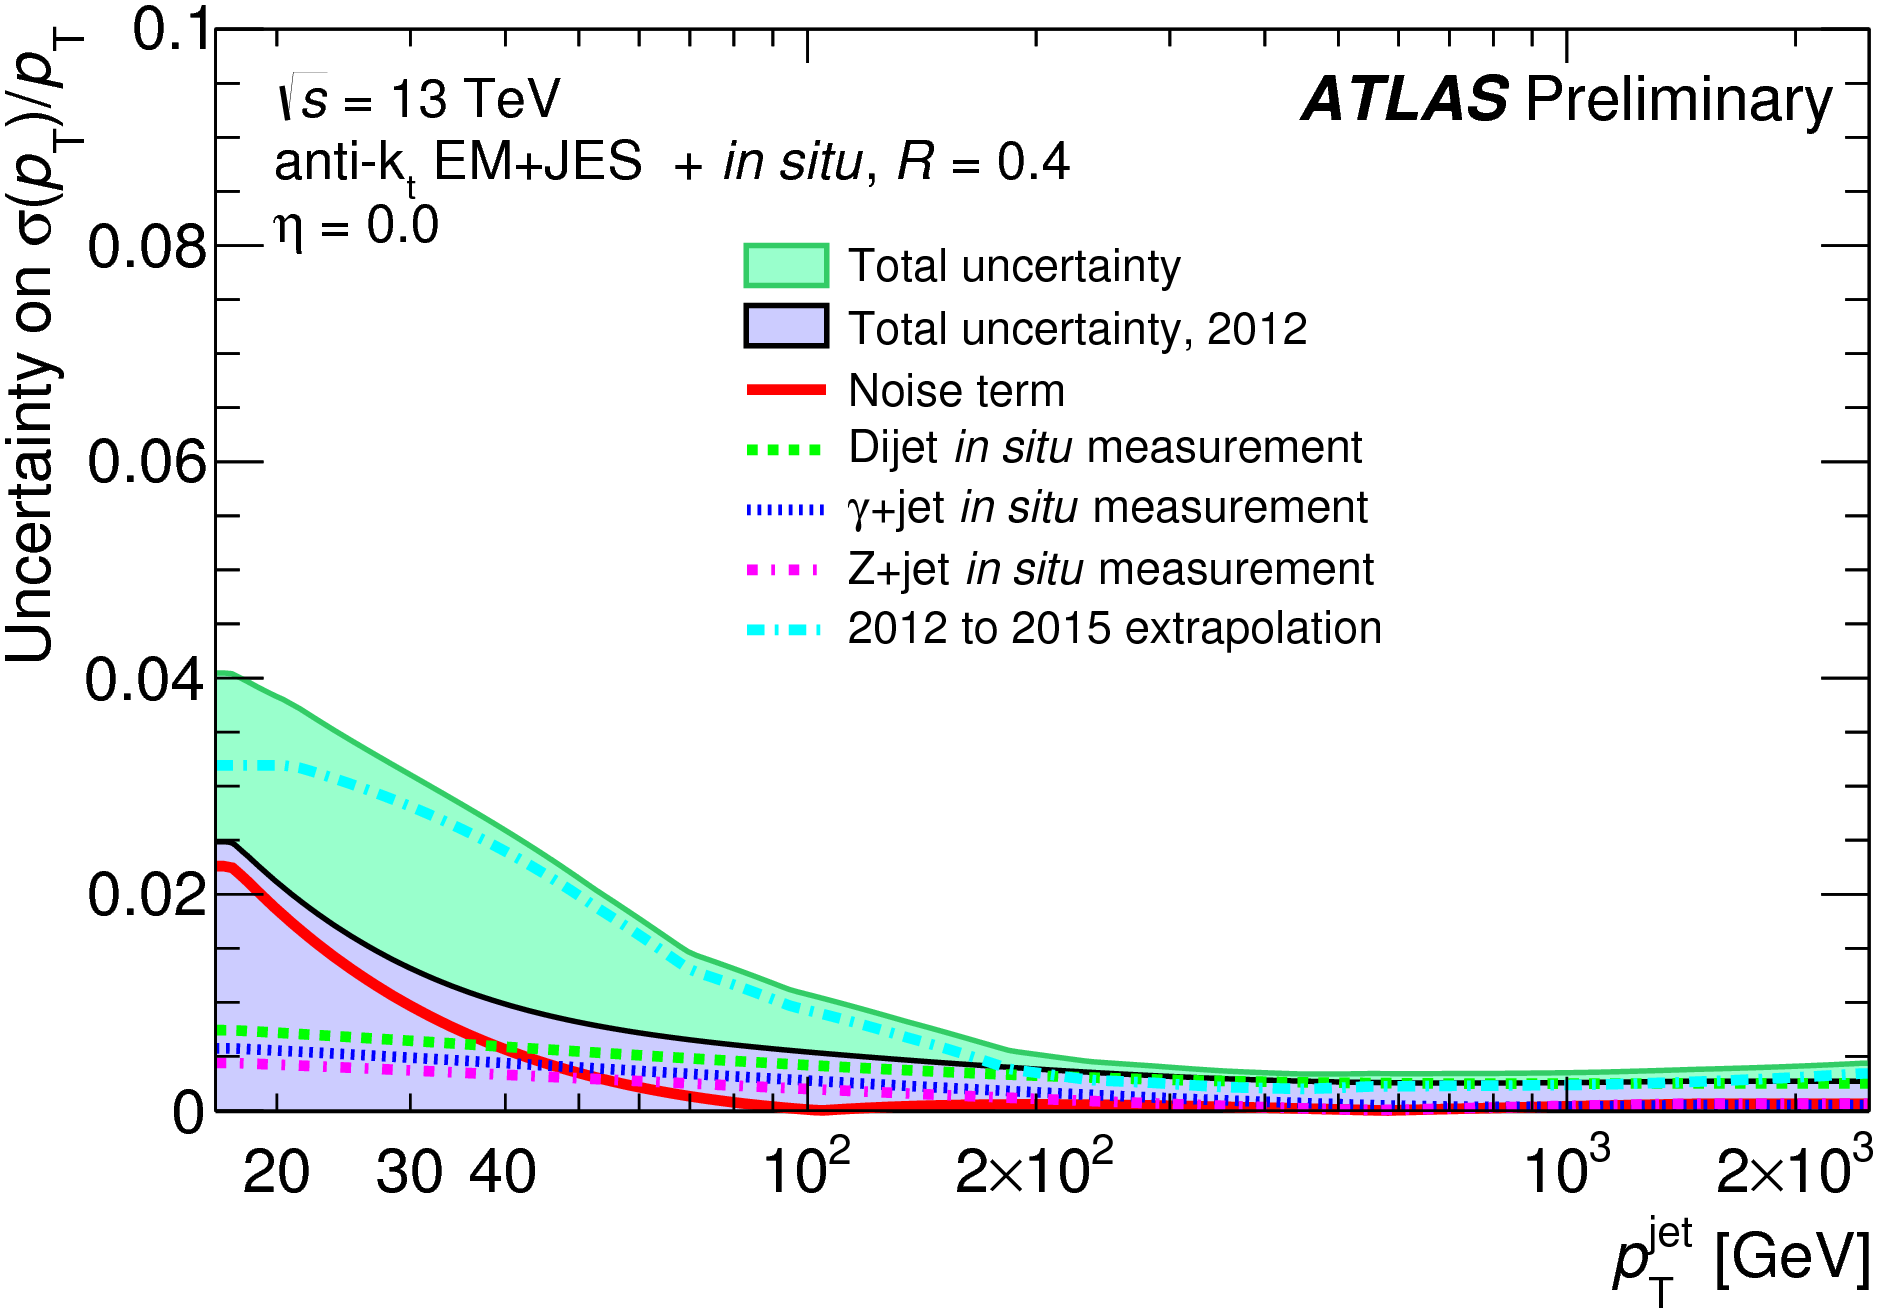
\includegraphics[width=0.48\textwidth]{figures/JetCalib/JER_pt.png}
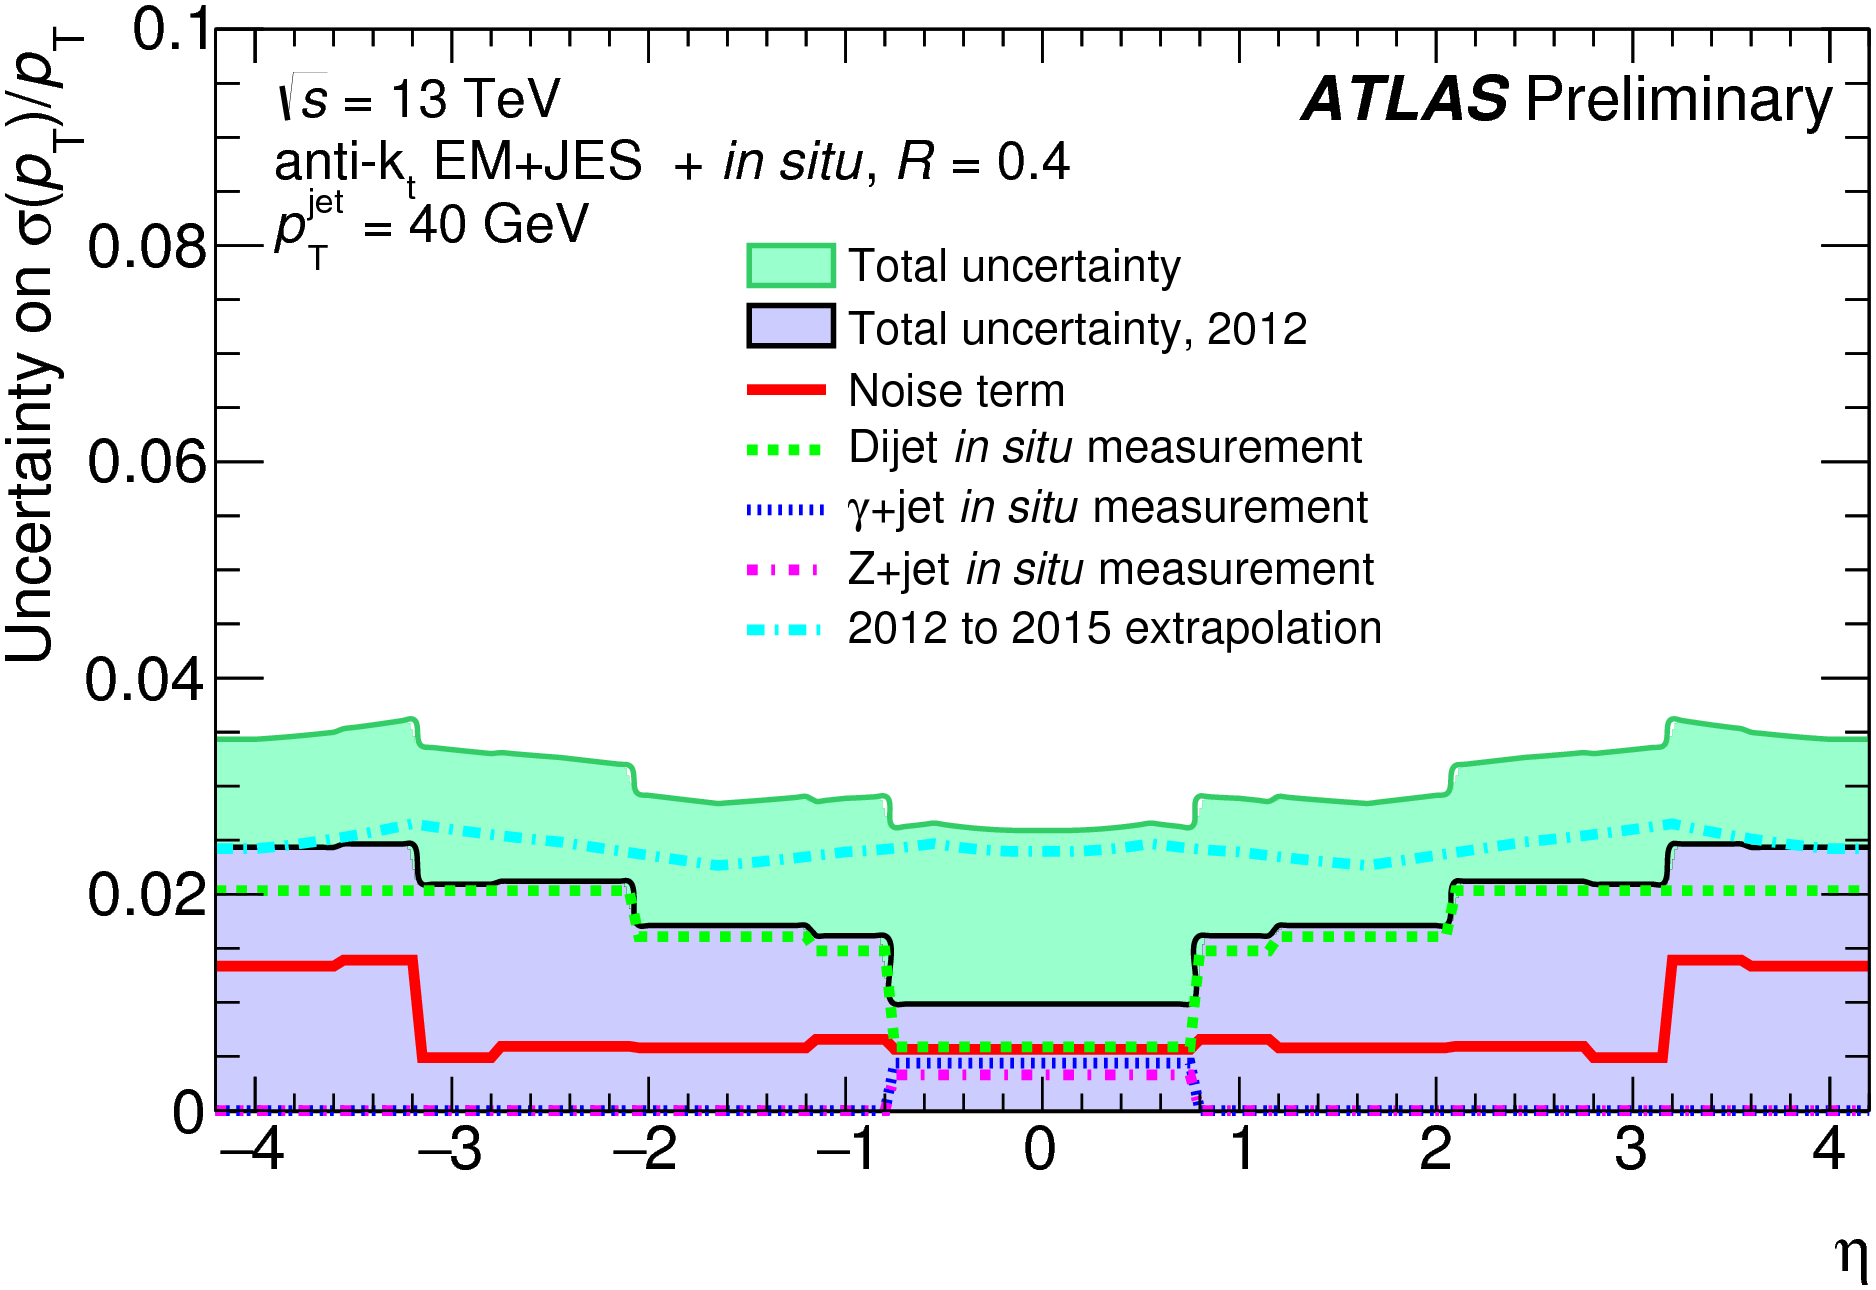
\includegraphics[width=0.48\textwidth]{figures/JetCalib/JER_eta.png}
\caption{Fractional uncertainty on the jet energy resolution (JER) vs jet $\eta$ and jet $\pt$.  }
\label{fig:sys:JES}
\end{center}
\end{figure}

\subsubsection*{Uncertainty on $b$-tagging}

\indent Uncertainties on $b$-tagging do not contribute a large systematic uncertainty to our analysis because we only require one b-tagged jet with a high $\pt$ requirement of 40 $\gev$.  At the same time, there is little extrapolation between background CRs and SR. The ttbar, $W$+jets and QCD multijets all use CRs that also require one $b$-tagged jet.  After fitting to CRs, $b$-tagging systematics amount to only 1-3 percent total uncertainty in SR.  \\

\indent  The $b$-tagging uncertainty is derived by the ATLAS flavor-tagging working group.  A separate set of weights are applied for each set of $b$-tagging variations.  These include scale factors on $b$-tagging efficiencies and the rate of mis-tagging of $c$-jets and light-flavored jets. \\

\subsubsection*{Uncertainty on the $\met$ Soft Term}

\indent  The majority of the uncertainty on $\met$ has already been accounted for by systematics on other reconstructed objects because the $\met$ is built out of fully calibrated and reconstructed physics objects.  However, there is one part of $\met$ reconstruction that does not come from any hard physics object; the $\met$ soft term.  Therefore, uncertainty on the $\met$ soft term forms an independent systematic uncertainty.  \\

\indent The uncertainty on the resolution and scale of the $\met$ soft term is derived by the ATLAS Jet/$\met$ group using two in-situ methods using $Z\rightarrow \mu\mu$ events.\cite{METPerform} The uncertainty on the $\met$ track soft term (TST) vs the number of reconstructed primary vertexes in $\ttbar$ simulation is shown in figure \ref{fig:sys:MET_TST_tt}. \\

\begin{figure}[!htbp]
\begin{center}
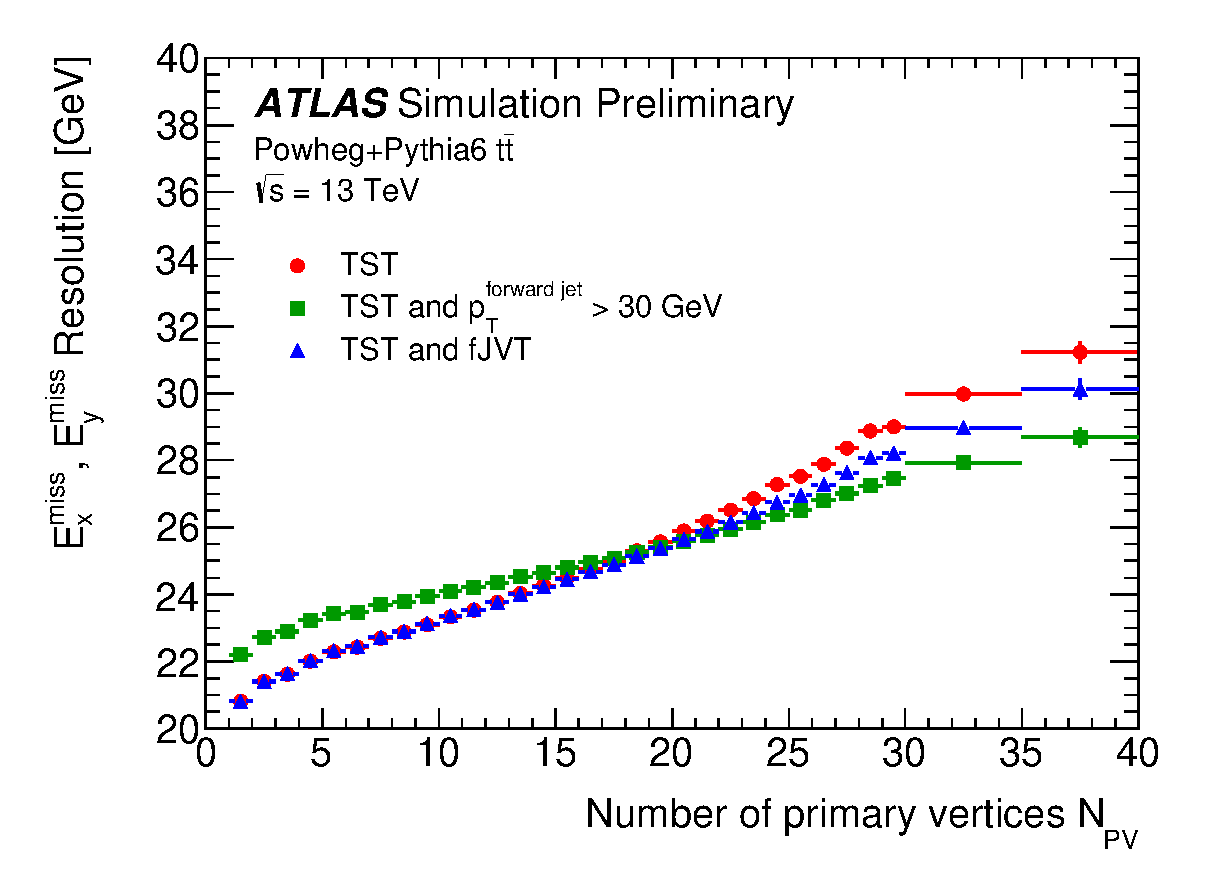
\includegraphics[width=0.48\textwidth]{figures/METCalib/MET_TST_tt.eps}
\caption{Uncertainty on the $\met$ track soft term (TST) vs the number of reconstructed vertexes.  }
\label{fig:sys:MET_TST_tt}
\end{center}
\end{figure}

\indent The $\met$ soft term resolution and scale uncertainty contribute a $1-2\%$ uncertainty on the total background yield.  The small uncertainty result from the high required $\met$ of at least 250 $\gev$ and little to no extrapolation across $\met$ between CR and SR for all major backgrounds. \\

\subsubsection*{Uncertainty on Lepton Reconstruction Efficiencies and Energy Scale}

\indent Uncertainty on lepton reconstruction and identification propagate to uncertainty on CR and SR yields.  These uncertainties include uncertainties on e/$\gamma$ resolution, energy scale, and reconstruction efficiency and muon momentum and reconstruction efficiency.  Lepton trigger scale factors are also taken into account for the $\ttbar+\gamma$ control region. \\

\indent These uncertainties are derived by the ATLAS E/$\gamma$ and muon combined performance groups and result in sub 1\% uncertainty on signal region yields.\cite{MuonReco,EleID} \\

\subsubsection*{Pileup}

\indent The uncertainty on the amount of pileup in 2015 and 2016 ATLAS data is estimated using a two sided variation in event weights.  One set of weight simulate a lower rates of pile-up interactions and the other simulate a higher rate.  Pile-up uncertainty contributes a 1-2\% uncertainty on the total background yield in the SR.



  % The detector systematic uncertainties above are calculated as the variations in the shapes of the original normalized histograms using ${\tt overallNormHistoSys}$ inside ${\tt HistFitter}$.
% \item{\bf Luminosity}
%The uncertainty of 2.8 $\%$ is assigned for the integrated luminosity and is denoted by {\bf Lumi} in the fit.


  %%%%%%%%%%%%%%%%%%%%%%%%%%%%%%%%%%%%%%%%%%%%%%%%%%%%%%%%%%
  %% Commented out for the time being since the est, method are not fully defined yet
  %%%%%%%%%%%%%%%%%%%%%%%%%%%%%%%%%%%%%%%%%%%%%%%%%%%%%%%%%%
%% \item{\bf Z fit method for $Z+jets$ background}
%% Following the detailed study in Section~\ref{section:Z_Results}, the uncertainty of 17
%% $\%$ is assigned to $Z+jets$ background for the $Z+jets$ fit-method estimation and is denoted by {\bf methodSysZ} in the fit.

%% \item{\bf Jet-smearing estimation method for multi-jet background}
%% The uncertainty of 100 $\%$ to is conservatively assigned to the
%% multi-jet yields for the jet-smearing estimation method and is denoted by
%% {\bf theoSysQCD} in the fit.

%% \item{\bf \dphimettrk\ and tau veto}
%%   No additional uncertainty is assigned for the requirements on
%%   \dphimettrk\ and on the tau veto. Both were discussed extensively for
%%   the 7 \TeV\ analysis \cite{7TeVSupportNote} where no additional
%%   systematic was assigned.  There are currently no official
%%   recommendations from the jet/etmiss group for \mettrk.  For the 7
%%   \TeV\ analysis, Fig 42 in Appendix C showed good agreement between
%%   data and MC for \dphimettrk\ in the tau-veto-inverted validation
%%   region.  For the current analysis, Fig. \ref{fig:SRA_dataMC} shows
%%   good agreement for the \mettrk\ variables in a \ttbar\ dominated
%%   region.  Tau veto systematics are documented in Appendix D of the 7
%%   \TeV\ note.  Data/MC comparisons were made for several variables in
%%   the 1-lepton control region and in the tau-veto-inverted validation
%%   region.  The tau fake rate was determined in a $Z\nu\nu$+jets
%%   dominated sample to be around 12\%. The systematic on this fake rate
%%   was determined with a study of the track multiplicity in jets; the
%%   track multiplicity for ($n_{trk} \le 4$) showed agreement within 5\%
%%   between data and MC.

  %%%%%%%%%%%%%%%%%%%%%%%%%%%%%%%%%%%%%%%%%%%%%%%%%%%%%%%%%%
  %%%%%%%%%%%%%%%%%%%%%%%%%%%%%%%%%%%%%%%%%%%%%%%%%%%%%%%%%%
  

  



\section{Theoretical Uncertainties}
\label{sec:TheoSystematics}

\indent Theoretical uncertainties quantify the uncertainty associated with MC generation including different scale parameters such as QCD renormalization, factorization scales and calculations on the matrix element and parton shower.  We vary MC generation with respect to the default setting and get different MC yields in the control and signal regions.  Because the background rate is normalized to the data in the control region, only differences in the transfer factor (defined in equation \ref{eqn:TF}) will result in a different signal region background prediction.    \\

\begin{equation}
T = \frac{N_{MC}^{SR}}{N_{MC}^{CR}}
\label{eqn:TF}
\end{equation}

\indent $N_{MC}^{SR}$ is the MC yield in the signal region and $N_{MC}^{CR}$ is the MC yield in the control region. \\

\indent  We determine the variation in the signal region background prediction according to the variation in the transfer factor as defined in equation \ref{eq:theory_uncertainty}.   All theoretical uncertainties for different backgrounds are assumed to be independent of one another.  \\

 \begin{eqnarray}
    \Delta_{X} = \frac{T_f^{\mathrm{up}} - T_f^{\mathrm{down}}}{T_f^{\mathrm{up}} + T_f^{\mathrm{down}}}
    \label{eq:theory_uncertainty}
  \end{eqnarray}

\indent $T_f^{\mathrm{up}}$ ($T_f^{\mathrm{down}}$) is the transfer factor defined in equation \ref{eqn:TF} for the upward (downward) variation in the systematics and $\Delta_{X}$ is the uncertainty due to parameter $X$ in the signal region.  \\

\subsection{$\ttbar$ Theoretical Uncertainty}
\label{sec:systTheo:ttbar}

\indent Theoretical uncertainties on $\ttbar$ production include uncertainties on the hard scattering matrix element calculation, uncertainties on the parton shower, and uncertainty on the amount of ISR/FSR produced in association with $\ttbar$.  \\

%\indent The $\ttbar$ ISR/FSR uncertainty is estimated by performing the analysis on fully reconstructed simulation with variations on the PS tuning and ME+PS matching scales that induces more/less ISR and FSR in the simulation. 

\indent  The $\ttbar$ ISR/FSR uncertainty is estimated by producing $\powheg\pythia$ MC samples with a different amount of radiation than the nominal MC sample.  These ISR/FSR variation samples are called the radHi and radLo samples.  In general, the radHi (radLo) sample generates a higher (lower) differential cross-section for $\ttbar$ that is produced in conjunction with hard ISR. \\

\indent The radHi and radLo samples are produced with different renormalization and factorization scales compared to the nominal sample (x0.5 to radHi and x2 to radLo).   The radHi sample also increase the $h_{damp}$ parameter which controls the matching between the parton shower and matrix element calculations.  The $h_{damp}$ parameter is increased from the nominal $m_{t}$ to $2 \times m_{t}$ for the radHi sample.   \\

\indent The $\ttbar$ ISR/FSR uncertainty ($ \Delta_{\ttbar ISR/FSR} $) is estimated using equation \ref{eq:ttbar_ISRuncert} where $T_f^{\mathrm{radHi}}$ ($T_f^{\mathrm{radLo}}$) is the transfer factor corresponding to the radHi (radLo) sample. \\

\begin{eqnarray}
    \Delta_{\ttbar ISR/FSR} = \frac{T_f^{\mathrm{radHi}} - T_f^{\mathrm{radLo}}}{T_f^{\mathrm{radHi}} + T_f^{\mathrm{radLo}}}
    \label{eq:ttbar_ISRuncert}
\end{eqnarray}

%\indent The uncertainty on the ME calculation and on the PS calculation is estimated by performing the analysis on truth level-simulation using different MC generator programs.  In short, the ISR/FSR uncertainty determines how much the $\ttbar$ yields in the signal region differ if different $\powheg$ and $\pythia$ settings were used.  The $\ttbar$ hard scattering and PS variations determines how much the $\ttbar$ yields in the signal region differ if different generator programs and parton shower tunes are used. \\

\indent Uncertainties on the hard scattering and parton shower are calculated by comparing the nominal $\powheg\pythia$ $\ttbar$ sample with the $\powheg\herwigpp$ $\ttbar$ and $\sherpa$ 2.2.1 $\ttbar$ samples.  The $\powheg\herwigpp$ sample has the same matrix element calculation as the nominal sample but uses $\herwigpp$ to perform a different set of parton shower calculation with a distinct parton shower tune.  The $\sherpa$ 2.2.1 $\ttbar$ sample perform a different matrix element and parton shower calculation using a different PDF set and parton shower tune.  More details on the different $\ttbar$ MC generation can be found in section \ref{sec:MC:Bkg}. \\

\indent We take an envelope of the $\sherpa$ and $\powheg\herwigpp$ variations as the combined $\ttbar$ hard scattering and parton shower uncertainty.  This is because the $\powheg\herwigpp$ and $\sherpa$ samples both vary the parton shower calculations.  Taking an envelope of both variations instead of summing the two in quadrature avoids double counting the parton shower uncertainty. The total hard scattering plus parton shower uncertainty is defined as the maximum of equation \ref{eq:ttbar_ME_uncertainty} and \ref{eq:ttbar_PS_uncertainty}.  \\

    \begin{eqnarray}
      \Delta_{\mathrm{hard~scatter}} = \frac{T_f^{\mathrm{\powheg\pythia}} - T_f^{\mathrm{\sherpa}}}{T_f^{\mathrm{\powheg\pythia}}}
      \label{eq:ttbar_ME_uncertainty}
    \end{eqnarray}

    \begin{eqnarray}
      \Delta_{\mathrm{PS}} = \frac{T_f^{\mathrm{\powheg\pythia}} - T_f^{\mathrm{\powheg\herwigpp}}}{T_f^{\mathrm{\powheg\pythia}}}
      \label{eq:ttbar_PS_uncertainty}
    \end{eqnarray}

\indent $T_f^{\mathrm{\powheg\pythia}}$, $T_f^{\mathrm{\powheg\herwigpp}}$ and $T_f^{\mathrm{\sherpa}}$ correspond to the transfer factors derived by using the nominal $\powheg\pythia$ $\ttbar$ MC, the $\powheg\herwigpp$ $\ttbar$ MC and the $\sherpa$ $\ttbar$ MC.  $\Delta_{\mathrm{hard~scatter}}$ is the uncertainty on the hard scattering calculation and $\Delta_{\mathrm{PS}}$ is the uncertainty on the parton shower calculation. \\

\indent The MC $\ttbar$ yields in the control region, validation region and signal region for the different $\ttbar$ samples and the $\ttbar$ theory uncertainties are given in Table \ref{tab:ttbar_unc_SRC}.  \\

\pagebreak
  
 \begin{table}[!h]
    \caption{MC yields and theory uncertainties for the $\ttbar$\ background for the control, validation and signal regions.  MC yields are quoted for before any fitting to the data in the control region. Uncertainties are derived using variations in the transfer factor according to equations \ref{eq:ttbar_ISRuncert}, \ref{eq:ttbar_ME_uncertainty} and \ref{eq:ttbar_PS_uncertainty}. The uncertainties are symmetrical and are quantified as percentage of total background yield. }
    \label{tab:ttbar_unc_SRC}
    \begin{center} %\footnotesize
    
        \begin{tabular}{|c|c|c|c|c|}
	\noalign{\smallskip}\noalign{\smallskip}\hline
        & CRTopC & VRTopC & SRC1 & SRC2\\
        \hline
$\ttbar$ (nominal)&   $668\pm 9 $&         $232\pm 5 $ &    $16.7\pm 1.6 $&         $31.7\pm 2.1 $\\
$\ttbar$ (rad up)&          $872\pm 11 $&         $293\pm 7 $ &            $25.2\pm 2.3 $&         $39.5\pm 2.3 $\\
$\ttbar$ (rad down)&        $521\pm 9 $&   $187\pm 5 $ &         $10.1\pm 1.0 $&         $19.2\pm 1.6 $\\
$\ttbar$ (Powheg+H++)&      $621\pm 10 $&         $206\pm 5 $&      $16.3\pm 1.8 $&         $27.8\pm 1.8 $\\
%$\ttbar$ (aMC@NLO+P8)&      $310\pm 60 $&          $113\pm 34 $&       $6\pm 5 $&      $<0.01$\\
$\ttbar$ (Sherpa)&          $840\pm 40 $&        $297\pm 30 $&            $30\pm 8 $&     $42\pm 9 $\\        
        \hline
        \multicolumn{3}{c}{\bf Transfer factors (in \%)} \\ \hline
        ISR/FSR &  &    $3.3$&      $20$&   $10$\\
        PS &     &   $4$&   $5$&    $6$\\
%        Generator (aMC@NLO) &  &          $46$&     $2$&   $32$\\
        Generator (Sherpa) &    &          $2$&    $40$&   $5$\\
        \hline       
        \end{tabular}
    
      \begin{tabular}{|c|c|c|c|}
	\noalign{\smallskip}\noalign{\smallskip}\hline
          & SRC3 & SRC4 & SRC5 \\
        \hline
$\ttbar$ (nominal) &         $21.7\pm 1.6 $&         $6.3\pm 0.8 $&          $0.60\pm 0.23 $\\
$\ttbar$ (rad up)&         $28.7\pm 2.1 $&         $8.6\pm 1.0 $&  $1.05\pm 0.33 $\\
$\ttbar$ (rad down)&         $15.8\pm 1.5 $&         $6.3\pm 1.2 $&  $0.7\pm 0.4 $\\
$\ttbar$ (Powheg+H++)&         $18.0\pm 1.5 $&         $6.5\pm 0.9 $&  $0.46\pm 0.18 $\\
%$\ttbar$ (aMC@NLO+P8)&        $4\pm 7 $&      $1\pm 5 $&      $0.9\pm 0.9 $\\
$\ttbar$ (Sherpa)&     $22\pm 5 $&     $7.4\pm 3.2 $&          $<0.01$\\        
        \hline
        \multicolumn{4}{c}{\bf Transfer factors (in \%)} \\ \hline
        ISR/FSR  &   $4$&    $10$&   $5$\\
        PS &    $11$&   $11$&   $20$\\
%        Generator (aMC@NLO) &          $15$&   $39$&   $40$\\
        Generator (Sherpa)  &    $19$&   $10$&   $100$\\
        \hline       
        \end{tabular}
       
        
    \end{center}
  \end{table}

\subsection{$\Wjets$ Theoretical Uncertainty}

\indent The $\sherpa$ generator is used to estimate $\Wjets$ theory uncertainties.  Variations of the renormalization and factorization scales are included.  The uncertainty for each variation is quantified as the uncertainty on the transfer factor according to equation \ref{eq:theory_uncertainty}.  The total $W$+jets theory uncertainty is the combination of all uncertainties summed in quadrature. \\

\indent The total theory uncertainty on $\Wjets$ in the signal region is given in Table \ref{tab:WThSyst}.  Values are given as percent uncertainties on $\Wjets$ yields in the signal region.  The uncertainties are symmetrical. \\

  \begin{table}[!h]
    \caption{Summary of the theory uncertainties (in percent) on $W$ production obtained using variations on transfer factors. The uncertainties are symmetrical and are quantified as percentage of total background yield.}
    \label{tab:WThSyst}
    \begin{center} %\footnotesize
    \begin{tabular}{|c|c|} \hline
{\bf SR} & {\bf uncertainty (\%)} \\ \hline
%SRA-TT & 9.5\\ \hline
%SRA-TW & 8.0\\ \hline
%SRA-T0 & 6.1\\ \hline
%SRB-TT & 9.1\\ \hline
%SRB-TW & 7.9\\ \hline
%SRB-T0 & 3.3\\ \hline
%SRC1 & 11.4\\ \hline
SRC1 & 12.5\\ \hline
SRC2 & 11.8\\ \hline
SRC3 & 10.7\\ \hline
SRC4 & 9.5\\ \hline
SRC5 & 11.3\\ \hline
%SRD-low & 8.8\\ \hline
%SRD-high & 8.2\\ \hline
%SRE & 9.5\\ \hline
%VRW & 1.9\\ \hline
\end{tabular}

    \end{center}
  \end{table}        

\subsection{Single-top Theoretical Uncertainty}

\indent Single-top theoretical uncertainties include the uncertainties on the parton shower, ISR/FSR, and the interference between $\ttbar$ and single-top in the Wt channel.  Single-top uncertainties are evaluated for the $Wt$ subprocess because the $Wt$ subprocess dominates the single-top background in the signal region.  A Feynman diagram for $Wt$ production is given in Figure \ref{fig:ST:feyn}.\\

\begin{figure}[h!]
\begin{center}
	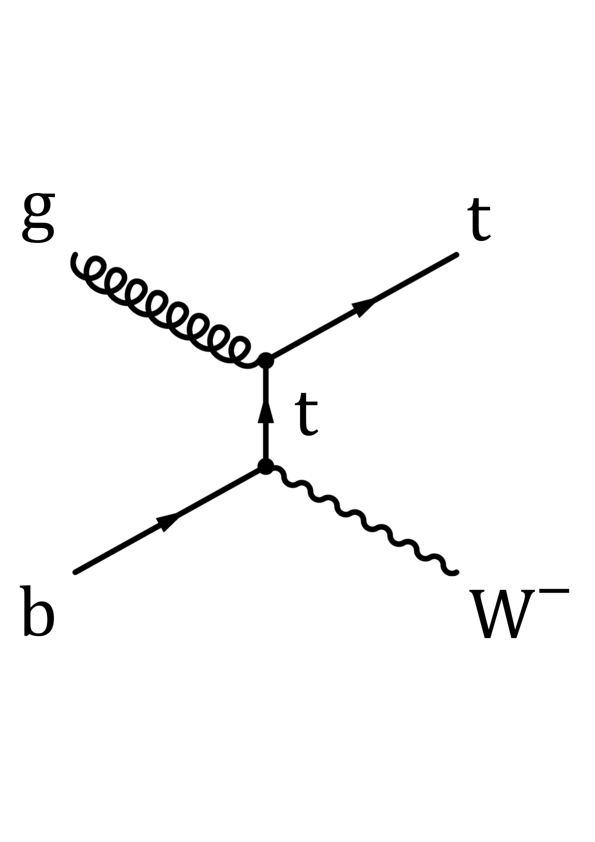
\includegraphics[width=0.45\textwidth]{figures/feynDiag/tW_chan.png}
\end{center}
\caption[Single top production Feynman diagram for the $Wt$ channel.]{Single top production Feynman diagram for the $Wt$ channel. }
\label{fig:ST:feyn}
\end{figure}

\indent The single-top parton shower uncertainty is modeled by comparing the nominal $\powheg\pythia$ sample with a $\powheg\herwigpp$ single-top sample in a similar fashion to the $\ttbar$ parton shower uncertainty in section \ref{sec:systTheo:ttbar}.  \\

\indent The single-top ISR/FSR uncertainty is also modeled by comparing the radHi and radLo $\powheg\pythia$ single-top samples to the nominal $\powheg\pythia$ samples.  This method is completely analogous to the modeling of the $\ttbar$ ISR/FSR uncertainty. \\

\indent The single-top interference uncertainty refers to the fact that there is an uncertainty in how to treat the interference between single-top and SM $\ttbar$.  The NLO calculation of the $pp \rightarrow Wt$ process will include contributions from $ pp \rightarrow \ttbar \rightarrow t + b + W$ process which is already included in the SM $\ttbar$.  In order to avoid double counting with SM $\ttbar$, we can subtract out the $pp \rightarrow \ttbar \rightarrow t + b + W$ contribution.  \\

\indent However, it is uncertain whether this subtraction should be done at either the amplitude level (DR scheme) or at the matrix element level (DS scheme).  Subtracting at the matrix element level also removes any potential interference between the single-top $pp \rightarrow Wt$ and the $ pp \rightarrow \ttbar \rightarrow t + b + W$ processes.  Subtracting at the amplitude level does not remove those interferences. \\

\indent  Both the DR and DS schemes violate formal gauge invariance and there is no consensus on the correct procedure to treat the single-top and  $\ttbar$ interference.  We quantify the interference uncertainty by taking the difference between the DR and DS schemes.  At the moment we take an 100\% interference uncertainty because of the low MC statistics in DS scheme. \\

\indent The single-top MC yields and theory uncertainties are given in Table \ref{tab:single_top_unc3}.  The MC yields corresponding to different single-top MC samples are given for control, validation and signal regions.  The single-top theory uncertainties are derived using transfer factors. \\

   \begin{table}[!h]
    \caption{Summary of the single-top (ST) theory uncertainties obtained in each of the signal regions. The uncertainties are computed according to the variation on the transfer factor defined in equation \ref{eq:theory_uncertainty}. The uncertainties are symmetrical and are quantified as percentage of total background yield. %The total uncertainty is the sum in quadrature of the uncertainties labeled ``Total    generator+PS+interference''. 
}
    \label{tab:single_top_unc3}
    
    \begin{center}% \footnotesize

       \begin{tabular}{|c|c|c|c|c|}
       \noalign{\smallskip}\noalign{\smallskip}\hline
        & CRST & VRTopC & SRC1 & SRC2 \\ \hline
         \hline
          ST (nominal) &          $41.7\pm 1.1$ &         $19.9\pm 0.8$ &          $0.66\pm 0.14$&         $1.14\pm 0.18$\\
          ST (radHi)&   $50.4\pm 1.3$ &         $21.9\pm 0.8$ &          $0.60\pm 0.14$&         $1.26\pm 0.20$\\
ST  (radLo)&   $34.9\pm 1.0$ &         $16.9\pm 0.7$ &          $0.57\pm 0.13$&         $0.77\pm 0.15$\\
ST (Powheg+H++)&       $39.2\pm 1.0$ &         $18.7\pm 0.7$ &          $0.62\pm 0.13$&         $0.84\pm 0.16$\\
ST  (DS)&       $6.8\pm 0.4$ &       $4.39\pm 0.31$ &   $0.12\pm 0.05$&         $0.30\pm 0.09$\\
          \hline \hline 
          \multicolumn{5}{c}{\bf Transfer factors (in \%)} \\ \hline
          ISR/FSR& &      $5.4\pm3.4$&       $16\pm17$&      $6\pm13$\\
          PS &  &      $0\pm7$ &     $0\pm30$&       $22\pm22$\\
          Interference (DR vs DS) &  &      $35\pm13$ &      $10\pm50$&      $60\pm50$\\
          \hline
        \end{tabular}

        \begin{tabular}{|c|c|c|c|}
        \noalign{\smallskip}\noalign{\smallskip}\hline
        \hline
         & SRC3 & SRC4 & SRC5\\ \hline
         \hline
          ST (nominal&         $0.99\pm 0.17$&         $0.39\pm 0.11$&         $0.12\pm 0.06$\\
          ST  (radHi)&         $1.33\pm 0.21$&         $0.57\pm 0.14$&         $0.25\pm 0.09$\\
          ST (radLo)&         $0.77\pm 0.15$&         $0.37\pm 0.10$&         $0.09\pm 0.05$\\
	ST  (Powheg+H++)&         $0.79\pm 0.15$&         $0.38\pm 0.10$&         $0.08\pm 0.05$\\
	ST  (DS)&         $0.23\pm 0.08$&         $0.16\pm 0.06$&         $0.020\pm 0.020$\\
          \hline \hline 
          \multicolumn{4}{c}{\bf Transfer factors (in \%)} \\ \hline
          ISR/FSR&       $9\pm13$&       $3\pm18$&       $32\pm32$\\
          PS &      $15\pm24$&      $0\pm40$&       $30\pm70$\\
          Interference (DR vs DS)  &      $40\pm50$&      $150\pm110$&    $0\pm110$\\
          \hline
        \end{tabular}
        
    \end{center}

  \end{table}


\subsection{$\ttV$ Theoretical Uncertainty}

\indent The $\ttV$ theoretical uncertainty include scale variations and variations on the underlying event tuning.  An additional uncertainty on the difference between the $\ttbar\gamma$ and $\ttbar Z$ vector boson $\pt$ differential cross sections is added to the total $\ttV$ uncertainty due to the procedure of using $\ttbar+\gamma$ to estimate $\ttV$.  The $\sherpa$+OpenLoops program\cite{OpenLoops} is used to calculate $\ttbar \gamma$ and $\ttbar Z$ vector boson differential cross-sections to NLO accuracy.  The difference between $\sherpa$+OpenLoops and the nominal {\sc MadGraph5\_aMC\/@NLO} cross-sections is combined in quadrature with the variations on the scale and the underlying event tune to give the total $\ttV$ theoretical uncertainty. \\

\indent The $\ttV$ theoretical uncertainty is given in Table \ref{tab:ttbarZ_unc1}.  The systematic uncertainty maybe large for $\ttV$ production in the signal region but $\ttV$ comprise about 1\% of our expected background. Therefore uncertainties on the $\ttV$  process do not contribute significantly to the total background uncertainty in the analysis. \\

  \begin{table}[!h]
      \caption{Summary of the theory uncertainties (in percent) on $\ttV$ production obtained on the transfer factor. The uncertainties are symmetrical and are quantified as percentage of total background yield.}
    \label{tab:ttbarZ_unc1}
    \begin{center} %\footnotesize
      \begin{tabular}{c||c} \hline\hline
{\bf SR} & {\bf uncertainty (\%)} \\ \hline
SRA-TT & 15.1\\ \hline
SRA-TW & 9.9\\ \hline
SRA-T0 & 13.7\\ \hline
SRB-TT & 7.3\\ \hline
SRB-TW & 5.7\\ \hline
SRB-T0 & 3.5\\ \hline
SRC1   & 95.5\\ \hline
SRC2   & 20.6\\ \hline
SRC3   & 21.4\\ \hline
SRC4   & 36.6\\ \hline
SRC5   & 30.9\\ \hline
SRD-low & 12.3\\ \hline
SRD-high & 15.1\\ \hline
SRE & 55.0\\ \hline
\hline
\end{tabular}

    \end{center}
  \end{table}

\subsection{Dibosons Theoretical Uncertainty}

A 50\% theory uncertainty is applied to the dibosons MC estimate.

\subsection{$Z$+jets Theoretical Uncertainty}

A 50\% theory uncertainty is applied to the $\Zjets$ MC estimate.

%\subsection{Signal Theoretical Uncertainty}

%  {\color{red} Coming soon}
